\documentclass[11pt]{scrartcl}
\usepackage[utf8]{inputenc}
\usepackage{amsmath,amsfonts,amssymb,amsrefs,mathtools,amsthm}
\usepackage{enumerate}
\usepackage{graphicx}
\usepackage{multicol}
\usepackage[all]{xy}
\usepackage{tikz}
\usetikzlibrary{snakes,patterns}
\usetikzlibrary{decorations.pathreplacing,calligraphy}
\usepackage{caption}
\usepackage{cancel}

\usepackage[bookmarksnumbered, colorlinks, plainpages]{hyperref}
\hypersetup{colorlinks=true,linkcolor=red, anchorcolor=green, citecolor=cyan, urlcolor=blue, filecolor=magenta, pdftoolbar=true}
\usepackage[capitalise]{cleveref}

\newtheorem*{definition}{Definition}
\newtheorem{theorem}{Theorem}
\newtheorem{lemma}[theorem]{Lemma}
\newtheorem{proposition}[theorem]{Proposition}
\newtheorem{remark}[theorem]{Remark}
\newtheorem{corollary}[theorem]{Corollary}
\newtheorem{example}[theorem]{Example}
\newtheorem{problem}[theorem]{Problem}

\DeclareMathOperator{\atan2}{atan2}
\DeclareMathOperator{\Div}{div}

\title{The 19th Problem}

\author{A Leisurely Excursion}

\date{}

\begin{document}
\maketitle

Have you ever wondered why soap bubbles are spherical, or why soap films look like they are pulling themselves into the shape of the least possible area, or why the light moving through glass of varying density bends and curves to find the fastest route, not the straightest one.
\begin{figure}[h]
    \centering
    \includegraphics[width=0.5\textwidth]{SoapFilm.jpeg}
    \caption{A soap film on a wire frame.}
\end{figure}

In each case, nature is quietly solving an optimization problem. Something is being minimized, whether it is the area or the time. One thing to note is that even if the wire frame itself (the boundary) has sharp, jagged corners, the soap film suspended inside is perfectly smooth. It is definitely interesting to ponder on why the film develops no gaps, tears, or defects.\\

\textit{Why should this be true? And more importantly: must it always be true?}\\

Before answering this, let's rewind to the dawn of the $20^{th}$ century. In the International Congress of Mathematicians held at Paris in August 1900, the German Mathematician David Hilbert proposed $23$ problems, most of which would prove to be very influential in the coming century. \footnote{He actually had $24$ problems but he chose not to publish it.} 
\begin{figure}[h]
    \centering
    \includegraphics[width=0.5\textwidth]{Hilbert .jpg}
    \caption{David Hilbert (1862–1943)}
\end{figure}



While many of his problems arose due to the urge to understand the foundational bedrock of Mathematics like the continuum hypothesis, a few were inspired by physics. Belonging to the latter category is the topic of our blog, which is the $19^{th}$ problem. Hilbert was fascinated by the observation that physical principles, usually cast as variational problems (like the principle of least action), seemed to produce solutions of remarkable smoothness.

These are but special cases of a universal variational principle. Hilbert observed that such analytic solutions arise from minimizing functional integrals of the form:
\begin{equation}\label{eq:functional}
J(u) = \int_{B_1} F(\nabla u) \, dx,
\end{equation}
where the function \( F \) (often called the Lagrangian) is analytic and \textit{strictly convex}. In the language of linear algebra, convexity here means the Hessian matrix of \( F \) is positive definite (specifically, \(\det(D^2 F) > 0\)).\\

\textit{The question is this: If the energy function \( F \) is analytic, does it follow that the minimizing configuration \( u \) is also analytic?}\\


Intuitively, the answer seemed to be yes. To prove it, we translate the minimization problem into an equation. We know from single-variable calculus that if \( f(x) \) has a minimum at \( x_0 \), then \( f'(x_0) = 0 \). We apply the same logic here.

Suppose \( u(x) \) is the true solution. Imagine we distort this solution by adding a small "perturbation" \( \phi(x) \), scaled by a tiny number \( \epsilon \):
\[
u_\epsilon(x) = u(x) + \epsilon \phi(x).
\]

Since \( u \) is a minimizer, the derivative of the energy with respect to \( \epsilon \) must be zero at \( \epsilon = 0 \):
\[
\frac{d}{d\epsilon} J(u + \epsilon \phi) \bigg|_{\epsilon=0} = 0.
\]
\begin{figure}[h]
\centering
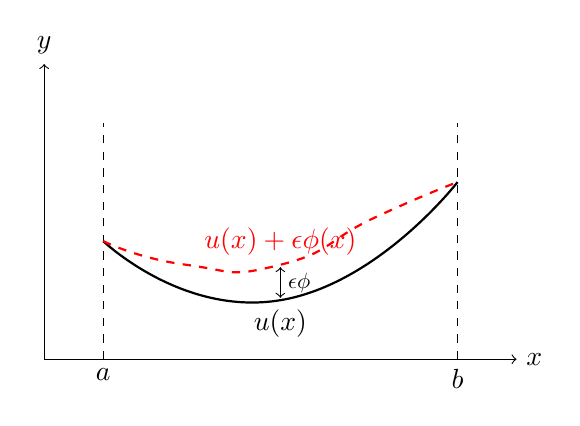
\begin{tikzpicture}[scale=1.5]
    % Axes
    \draw[->] (0,0) -- (4,0) node[right] {$x$};
    \draw[->] (0,0) -- (0,2.5) node[above] {$y$};

    % Domain boundaries
    \draw[dashed] (0.5,0) -- (0.5,2);
    \draw[dashed] (3.5,0) -- (3.5,2);
    \node[below] at (0.5,0) {$a$};
    \node[below] at (3.5,0) {$b$};

    % True Solution u(x) 
    \draw[thick, black] plot [smooth, tension=1] coordinates {(0.5,1) (2,0.5) (3.5,1.5)};
    \node[below] at (2,0.5) {$u(x)$};

    % Perturbed Solution
    \draw[thick, dashed, red] plot [smooth, tension=1] coordinates {(0.5,1) (1.2, 0.8) (2,0.8) (2.8, 1.2) (3.5,1.5)};
    \node[red, above] at (2,0.8) {$u(x) + \epsilon\phi(x)$};

    % Annotation
    \draw[<->] (2, 0.52) -- (2, 0.78);
    \node[right, scale=0.8] at (2, 0.65) {$\epsilon\phi$};

\end{tikzpicture}
\caption{}
\end{figure}

Calculating this (using the Chain Rule inside the integral) and integrating by parts gives the celebrated Euler-Lagrange equation:
\begin{equation}\label{eq:euler-lagrange}
\operatorname{Div}(\nabla F(\nabla u)) = 0.
\end{equation}

Now, we expand this. Applying the Chain Rule to the term \( \nabla F(\nabla u) \), we get:
\begin{equation}\label{eq:euler-lagrange-expanded}
\sum_{i,j=1}^n F_{ij}(\nabla u)\, u_{ij} = 0,
\end{equation}
where \( F_{ij} \) are entries of the Hessian of \( F \), and \( u_{ij} \) are the second partial derivatives of \( u \).

Here comes the trouble. If we differentiate \cref{eq:euler-lagrange-expanded} with respect to \( x_k \), letting \( v = u_{x_k} \), we obtain a linear elliptic equation for the partial derivatives of \( u \):
\begin{equation}\label{eq:linearized}
\sum_{i,j=1}^n \frac{\partial}{\partial x_i} \Big( a_{ij}(x) \frac{\partial v}{\partial x_j} \Big) = 0, \quad \text{where } a_{ij}(x) = F_{ij}(\nabla u(x)).
\end{equation}


\begin{figure}[h]
    \centering
    \includegraphics[width=0.5\textwidth]{Charles_Morrey_Jr.jpeg}
    \caption{Charles Morrey Jr. (1907–1984)}
\end{figure}



However, the coefficients
\(
a_{ij}(x) = F_{ij}(\nabla u(x))
\)
of this new linearized equation \cref{eq:linearized} depend intrinsically on the unknown gradient.
If we assume only that \( u \) has bounded slope so that the gradient \( \nabla u \) is bounded but not known to be
continuous, then these coefficients are bounded, but they may be discontinuous.
We are thus caught in a vicious circle: to prove the coefficients are smooth, we
need the solution's gradient to be smooth; but to prove the solution is smooth,
the classical theory demands the coefficients be smooth. This ``gap'' between
having a bounded slope versus a continuous slope was what Morrey later called the
``sad state of affairs'' that hindered progress for decades.


The solution was finally achieved by bridging this gap. Let us illustrate the strategy in 2D, using geometric intuition.

You are likely familiar with the gradient $\nabla u$ as a vector field pointing in the direction of steepest increase. But for this problem, we need a shift in perspective. Imagine mapping every point $x$ in our domain not to its height $u(x)$, but to its slope vector $\nabla u(x)$.
This creates a ``gradient map'' from the physical domain into a ``plane of slopes.''\\

\textit{The core question of regularity is simply: Is this map continuous? Or can the slope jump abruptly from one value to another, creating a sharp crease or kink in our soap film?}

\begin{figure}[h]
    \centering
    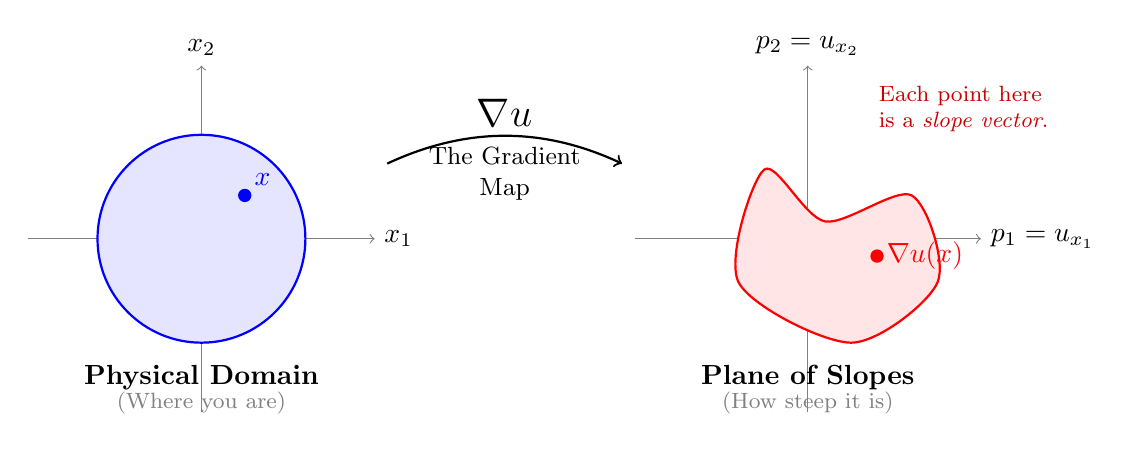
\begin{tikzpicture}[scale=1.1]
        % --- LEFT: PHYSICAL DOMAIN  ---
        \begin{scope}[shift={(-3.5,0)}]
            % Axes
            \draw[->, gray] (-2,0) -- (2,0) node[right, black] {$x_1$};
            \draw[->, gray] (0,-2) -- (0,2) node[above, black] {$x_2$};

            % Domain
            \filldraw[fill=blue!10, draw=blue, thick] (0,0) circle (1.2);
            \node at (0, -1.6) {\textbf{Physical Domain}};
            \node[font=\footnotesize, gray] at (0, -1.9) {(Where you are)};

            % A specific point x
            \filldraw[blue] (0.5, 0.5) circle (2pt) node[above right] {$x$};
        \end{scope}

        % --- MAPPING ARROW ---
        \draw[->, thick, shorten >= 5pt, shorten <= 5pt] (-1.5, 0.8) to[bend left=25] node[midway, above] {\Large $\nabla u$} node[midway, below, font=\small, align=center] {The Gradient\\Map} (1.5, 0.8);

        % --- RIGHT: PLANE OF SLOPES (Gradient Space) ---
        \begin{scope}[shift={(3.5,0)}]
            % Axes (p1, p2 represents slopes)
            \draw[->, gray] (-2,0) -- (2,0) node[right, black] {$p_1 = u_{x_1}$};
            \draw[->, gray] (0,-2) -- (0,2) node[above, black] {$p_2 = u_{x_2}$};

            % The Image (Distorted Blob)
            \filldraw[fill=red!10, draw=red, thick] plot [smooth cycle] coordinates {(0.2,0.2) (1.2,0.5) (1.5,-0.5) (0.5,-1.2) (-0.8,-0.5) (-0.5, 0.8)};

            \node at (0, -1.6) {\textbf{Plane of Slopes}};
            \node[font=\footnotesize, gray] at (0, -1.9) {(How steep it is)};

            % The Mapped Point p = Grad u(x)
            \filldraw[red] (0.8, -0.2) circle (2pt) node[right] {$\nabla u(x)$};

            % Annotation explaining the coordinates
            \node[align=left, font=\footnotesize, red!80!black] at (1.8, 1.5) {Each point here\\is a \textit{slope vector}.};
        \end{scope}
    \end{tikzpicture}
    \caption{\textbf{The Gradient Map.} This map takes a location $x$ in the physical domain (left) and sends it to its corresponding slope vector $\nabla u(x)$ in the plane of slopes (right). If the solution is smooth, the red "blob" of slopes will be connected. If the solution has a crease, this blob will be torn apart.}
    \label{fig:gradient_map}
\end{figure}

Imagine the image of the gradient map \( \nabla u \) as a region (a "blob") in the plane. Fix a direction \( e \) (a unit vector) and consider the strip in the gradient plane between two parallel lines perpendicular to \( e \), defined by values \( a < b \).
\\

Let 
\(
v(x) = \nabla u(x) \cdot e
\)
be the corresponding directional derivative. If the gradient image \( \nabla u(B_r) \) crosses this strip, it means \( v \) takes values both below \( a \) and above \( b \) within the ball \( B_r \).




\begin{figure}[h]
\centering

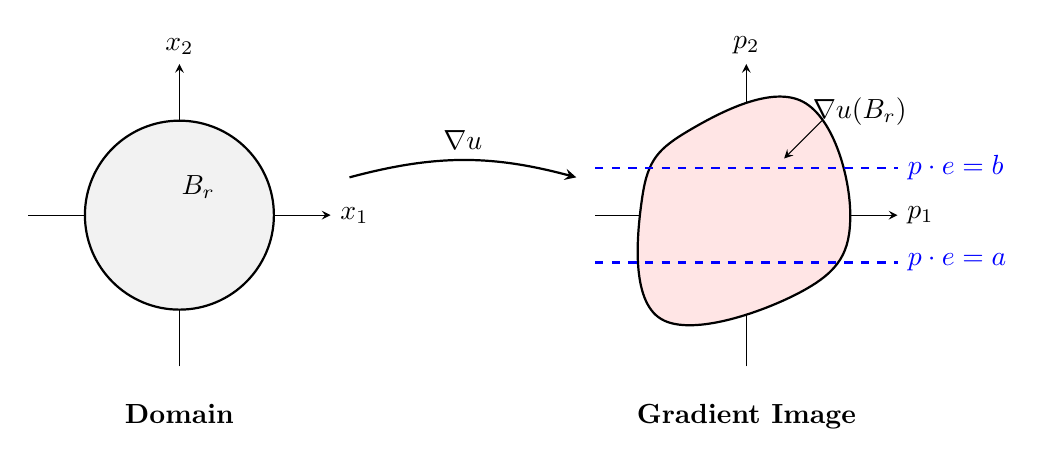
\begin{tikzpicture}[scale=1.2, >=stealth]

    %========================
    % Left Panel: Domain
    %========================
    \draw[->] (-1.6,0) -- (1.6,0) node[right] {$x_1$};
    \draw[->] (0,-1.6) -- (0,1.6) node[above] {$x_2$};

    \draw[thick, fill=gray!10] (0,0) circle (1);
    \node at (0.2,0.3) {$B_r$};

    \node[below] at (0,-1.9) {\textbf{Domain}};

    % Arrow
    \draw[->, thick]
        (1.8,0.4)
        to[bend left=15]
        node[midway, above] {$\nabla u$}
        (4.2,0.4);

    \begin{scope}[shift={(6,0)}]

        \draw[->] (-1.6,0) -- (1.6,0) node[right] {$p_1$};
        \draw[->] (0,-1.6) -- (0,1.6) node[above] {$p_2$};

        \draw[thick, fill=red!10]
        plot[smooth cycle, tension=0.7] coordinates {
            (-0.9,-1.1)
            (0.6,-0.8)
            (1.1,0)
            (0.6,1.2)
            (-0.6,0.9)
            (-1.1,0.2)
        };

        \node at (1.2,1.1) {$\nabla u(B_r)$};
        \draw[->] (0.8,1.0) -- (0.4,0.6);

        \draw[dashed, blue, thick]
            (-1.6,-0.5) -- (1.6,-0.5)
            node[right] {$p\cdot e = a$};

        \draw[dashed, blue, thick]
            (-1.6,0.5) -- (1.6,0.5)
            node[right] {$p\cdot e = b$};

        \node[below] at (0,-1.9) {\textbf{Gradient Image}};
    \end{scope}

\end{tikzpicture}

\caption{Chopping at the gradient image with lines}
\end{figure}





Here we use the Maximum Principle. The Maximum Principle is a powerful property of elliptic equations. You've seen a special case already: Laplace's equation 
\(
\nabla^2 u = 0.
\)
Its solutions (harmonic functions) obey the Mean Value Property and the Maximum Principle: the maximum and minimum occur on the boundary. Our linearized equation \cref{eq:linearized} is a generalization of Laplace's equation with variable coefficients \(a_{ij}(x)\). The principle still holds: the oscillation of \(v\) inside a ball is controlled by its oscillation on the boundary-like how the temperature at the center of a room is bounded by the temperatures on the walls.



In simple terms, for elliptic equations, the values inside a domain are controlled by the values on the boundary (much like temperature in a room is controlled by the walls).

By this principle, if \( v \) oscillates inside \( B_r \), it must oscillate at least as much on the boundary circle \( \partial B_r \). 
This allows us to restrict our attention to the boundary.

To see if this oscillation can persist as \( r \to 0 \), we quantify its "energy cost" using a geometric estimate:
\begin{equation}\label{eq:courant-lebesgue}
(\operatorname{osc}_{\partial B_r} v)^2 \le \frac{\pi}{\ln(1/2r)} \int_{B_{1/2}} |\nabla v|^2 \, dx.
\end{equation}
\footnote{ $\omega(r) := \operatorname{osc}_{\partial B_r} v$}

Suppose, for contradiction, that the oscillation stays large. Specifically, assume that on all circles \( \partial B_r \), the oscillation is bounded below by a constant \( \delta > 0 \).

Summing these oscillations (integrating with respect to \( r \)), due to the term \( \ln(1/r) \) , the required energy must diverge (recall the harmonic series):
\[
\text{Energy} \sim \int \frac{1}{r} \, dr \to \infty.
\]

However, we know there exists a finite upper bound. The differential equation itself provides a "natural" energy bound (Caccioppoli inequality):
\begin{equation}\label{eq:caccioppoli}
\int_{B_{1/2}} |\nabla v|^2 \, dx \le C \int_{B_1} v^2 \, dx < \infty.
\end{equation}

This is a contradiction: \cref{eq:courant-lebesgue} requires infinite energy, but \cref{eq:caccioppoli} bounds it finitely.

Therefore, for sufficiently small \( r \), the gradient image \( \nabla u(B_r) \) cannot cross the strip. It must lie entirely on one side. By "chopping" with strips in various directions, we force the gradient image to localize to a single point as \( r \to 0 \). Thus, \( \nabla u \) is continuous.\\







It is worth pausing to remark that this success in 2D relies on a "happy accident of geometry" - a special feature that disappears in higher dimensions. The linearized equation implies that the gradient map
\(
\nabla u: \mathbb{R}^2 \to \mathbb{R}^2
\)
behaves like a linear transformation with bounded distortion. Recall from linear algebra that a matrix \( A \) maps the unit circle to an ellipse. The "distortion" is determined by the condition number (the ratio of eigenvalues):
\begin{equation}\label{eq:distortion}
K = \frac{|\lambda_{\max}|}{|\lambda_{\min}|}.
\end{equation}



\begin{figure}[h]
\centering
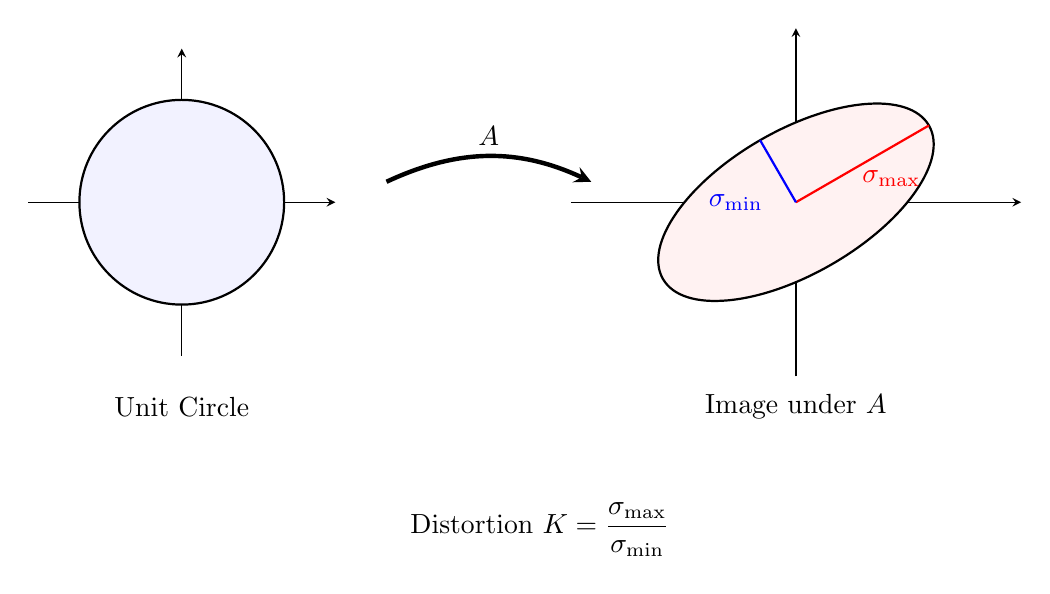
\begin{tikzpicture}[scale=1.3, >=stealth]

    % ---Unit Circle ---
    \begin{scope}
        \draw[->] (-1.5,0) -- (1.5,0);
        \draw[->] (0,-1.5) -- (0,1.5);
        \draw[thick, fill=blue!5] (0,0) circle (1cm);
        \node at (0,-2) {Unit Circle};
    \end{scope}

    % --- Transformation Arrow ---
    \draw[->, ultra thick] (2,0.2) to[bend left=25] node[midway, above] {$A$} (4,0.2);

    % --- Ellipse ---
    \begin{scope}[shift={(6,0)}]
        \draw[->] (-2.2,0) -- (2.2,0);
        \draw[->] (0,-1.7) -- (0,1.7);
        
        \draw[thick, fill=red!5, rotate=30] (0,0) ellipse (1.5cm and 0.7cm);
        
        % Semi-major axis
        \draw[thick, red, rotate=30] (0,0) -- (1.5,0);
        \node[red, above right=2pt] at (0.5,0) {$\sigma_{\max}$};
        
        % Semi-minor axis
        \draw[thick, blue, rotate=30] (0,0) -- (0,0.7);
        \node[blue, right=2pt] at (-1,0) {$\sigma_{\min}$};
        
        \node at (0,-2) {Image under $A$};
    \end{scope}

    % --- Bottom Text ---
    \node at (3.5, -3.2)
        {Distortion $K = \dfrac{\sigma_{\max}}{\sigma_{\min}}$};

\end{tikzpicture}

\caption{Action of a linear map on the unit circle and the induced distortion.}
\end{figure}

In 2D, the ellipticity condition in \cref{eq:linearized} forces this ratio to be bounded. We know that multiplying by a complex number corresponds to a matrix that only rotates and scales (it maps circles to circles, so $K=1$). The condition we have of $K < \infty$ forces the space to stay "close" to this ideal structure. It cannot flatten the circle into a line (which would mean $K \to \infty$). This geometric "rigidity" is the safety net: it prevents the gradient from tearing or becoming discontinuous.

This is the "accident": in 2D, the rigid structure of complex numbers prevents the gradient from tearing or becoming discontinuous. However, this is strictly a two-dimensional luxury. In 3D, there is no direct equivalent to complex numbers, and this geometric "safety net" vanishes.But while we have it, we use it. The "chopping" argument works because in 2D, a line cuts the plane in half. We can trap the oscillation. This grants us the precise rate of convergence. The scale invariance of our equation implies that if the oscillation drops by a factor on one scale, it must drop by the same factor on the next.

Mathematically, we obtain a recurrence relation for the oscillation \( \omega(r) \). If we shrink the radius by \( \delta \), the oscillation drops by half:
\begin{equation}\label{eq:recurrence}
\omega(\delta r) \le \frac{1}{2} \omega(r) \implies \omega(\delta^k) \le 2^{-k} \omega(1).
\end{equation}

This implies that the oscillation decays as a power of the radius:
\begin{equation}\label{eq:holder}
\omega(r) \le C r^\alpha.
\end{equation}

\Cref{eq:holder} guarantees that the gradient $\nabla u$ is continuous with a controlled rate of convergence (Hölder continuity). Thus, in the planar case, the specific geometry of 2D forces regularity. The wild oscillations are controlled by the very cost of their existence. While higher dimensions offer distinct (and much harder) challenges where this "happy accident" no longer applies, our excursion pauses here, having admired the clear view from the two-dimensional case.



\end{document}


